\documentclass{article}
\usepackage[margin=1in]{geometry}
\usepackage[linesnumbered,ruled,vlined]{algorithm2e}
\usepackage{amsfonts}
\usepackage{amsmath}
\usepackage{amssymb}
\usepackage{amsthm}
\usepackage{enumitem}
\usepackage{fancyhdr}
\usepackage{hyperref}
\usepackage{minted}
\usepackage{multicol}
\usepackage{pdfpages}
\usepackage{standalone}
\usepackage[many]{tcolorbox}
\usepackage{tikz-cd}
\usepackage{transparent}
\usepackage{xcolor}
% \tcbuselibrary{minted}

\author{Nathan Solomon}

\newcommand{\fig}[1]{
    \begin{center}
        \includegraphics[width=\textwidth]{#1}
    \end{center}
}

% Math commands
\renewcommand{\d}{\mathrm{d}}
\DeclareMathOperator{\id}{id}
\DeclareMathOperator{\im}{im}
\DeclareMathOperator{\proj}{proj}
\DeclareMathOperator{\Span}{span}
\DeclareMathOperator{\Tr}{Tr}
\DeclareMathOperator{\tr}{tr}
\DeclareMathOperator{\ad}{ad}
\DeclareMathOperator{\ord}{ord}
%%%%%%%%%%%%%%% \DeclareMathOperator{\sgn}{sgn}
\DeclareMathOperator{\Aut}{Aut}
\DeclareMathOperator{\Inn}{Inn}
\DeclareMathOperator{\Out}{Out}
\DeclareMathOperator{\stab}{stab}

\newcommand{\N}{\ensuremath{\mathbb{N}}}
\newcommand{\Z}{\ensuremath{\mathbb{Z}}}
\newcommand{\Q}{\ensuremath{\mathbb{Q}}}
\newcommand{\R}{\ensuremath{\mathbb{R}}}
\newcommand{\C}{\ensuremath{\mathbb{C}}}
\renewcommand{\H}{\ensuremath{\mathbb{H}}}
\newcommand{\F}{\ensuremath{\mathbb{F}}}

\newcommand{\E}{\ensuremath{\mathbb{E}}}
\renewcommand{\P}{\ensuremath{\mathbb{P}}}

\newcommand{\es}{\ensuremath{\varnothing}}
\newcommand{\inv}{\ensuremath{^{-1}}}
\newcommand{\eps}{\ensuremath{\varepsilon}}
\newcommand{\del}{\ensuremath{\partial}}
\renewcommand{\a}{\ensuremath{\alpha}}

\newcommand{\abs}[1]{\ensuremath{\left\lvert #1 \right\rvert}}
\newcommand{\norm}[1]{\ensuremath{\left\lVert #1\right\rVert}}
\newcommand{\mean}[1]{\ensuremath{\left\langle #1 \right\rangle}}
\newcommand{\floor}[1]{\ensuremath{\left\lfloor #1 \right\rfloor}}
\newcommand{\ceil}[1]{\ensuremath{\left\lceil #1 \right\rceil}}
\newcommand{\bra}[1]{\ensuremath{\left\langle #1 \right\rvert}}
\newcommand{\ket}[1]{\ensuremath{\left\lvert #1 \right\rangle}}
\newcommand{\braket}[2]{\ensuremath{\left.\left\langle #1\right\vert #2 \right\rangle}}

\newcommand{\catname}[1]{{\normalfont\textbf{#1}}}

\newcommand{\up}{\ensuremath{\uparrow}}
\newcommand{\down}{\ensuremath{\downarrow}}

% Custom environments
\newtheorem{thm}{Theorem}[section]

\definecolor{probBackgroundColor}{RGB}{250,240,240}
\definecolor{probAccentColor}{RGB}{140,40,0}
\newenvironment{prob}{
    \stepcounter{thm}
    \begin{tcolorbox}[
        boxrule=1pt,
        sharp corners,
        colback=probBackgroundColor,
        colframe=probAccentColor,
        borderline west={4pt}{0pt}{probAccentColor},
        breakable
    ]
    \color{probAccentColor}\textbf{Problem \thethm.} \color{black}
} {
    \end{tcolorbox}
}

\definecolor{exampleBackgroundColor}{RGB}{212,232,246}
\newenvironment{example}{
    \stepcounter{thm}
    \begin{tcolorbox}[
      boxrule=1pt,
      sharp corners,
      colback=exampleBackgroundColor,
      breakable
    ]
    \textbf{Example \thethm.}
} {
    \end{tcolorbox}
}

\definecolor{propBackgroundColor}{RGB}{255,245,220}
\definecolor{propAccentColor}{RGB}{150,100,0}
\newenvironment{prop}{
    \stepcounter{thm}
    \begin{tcolorbox}[
        boxrule=1pt,
        sharp corners,
        colback=propBackgroundColor,
        colframe=propAccentColor,
        breakable
    ]
    \color{propAccentColor}\textbf{Proposition \thethm. }\color{black}
} {
    \end{tcolorbox}
}

\definecolor{thmBackgroundColor}{RGB}{235,225,245}
\definecolor{thmAccentColor}{RGB}{50,0,100}
\renewenvironment{thm}{
    \stepcounter{thm}
    \begin{tcolorbox}[
        boxrule=1pt,
        sharp corners,
        colback=thmBackgroundColor,
        colframe=thmAccentColor,
        breakable
    ]
    \color{thmAccentColor}\textbf{Theorem \thethm. }\color{black}
} {
    \end{tcolorbox}
}

\definecolor{corBackgroundColor}{RGB}{240,250,250}
\definecolor{corAccentColor}{RGB}{50,100,100}
\newenvironment{cor}{
    \stepcounter{thm}
    \begin{tcolorbox}[
        enhanced,
        boxrule=0pt,
        frame hidden,
        sharp corners,
        colback=corBackgroundColor,
        borderline west={4pt}{0pt}{corAccentColor},
        breakable
    ]
    \color{corAccentColor}\textbf{Corollary \thethm. }\color{black}
} {
    \end{tcolorbox}
}

\definecolor{lemBackgroundColor}{RGB}{255,245,235}
\definecolor{lemAccentColor}{RGB}{250,125,0}
\newenvironment{lem}{
    \stepcounter{thm}
    \begin{tcolorbox}[
        enhanced,
        boxrule=0pt,
        frame hidden,
        sharp corners,
        colback=lemBackgroundColor,
        borderline west={4pt}{0pt}{lemAccentColor},
        breakable
    ]
    \color{lemAccentColor}\textbf{Lemma \thethm. }\color{black}
} {
    \end{tcolorbox}
}

\definecolor{proofBackgroundColor}{RGB}{255,255,255}
\definecolor{proofAccentColor}{RGB}{80,80,80}
\renewenvironment{proof}{
    \begin{tcolorbox}[
        enhanced,
        boxrule=1pt,
        sharp corners,
        colback=proofBackgroundColor,
        colframe=proofAccentColor,
        borderline west={4pt}{0pt}{proofAccentColor},
        breakable
    ]
    \color{proofAccentColor}\emph{\textbf{Proof. }}\color{black}
} {
    \qed \end{tcolorbox}
}

\definecolor{noteBackgroundColor}{RGB}{240,250,240}
\definecolor{noteAccentColor}{RGB}{30,130,30}
\newenvironment{note}{
    \begin{tcolorbox}[
        enhanced,
        boxrule=0pt,
        frame hidden,
        sharp corners,
        colback=noteBackgroundColor,
        borderline west={4pt}{0pt}{noteAccentColor},
        breakable
    ]
    \color{noteAccentColor}\textbf{Note. }\color{black}
} {
    \end{tcolorbox}
}


\fancyhf{}
\setlength{\headheight}{24pt}

\date{\today}
\title{Math 132 Homework \#5}

\begin{document}
\maketitle

\begin{prob}
    Chapter IV section 4 exercise 1(a)
\end{prob}
Let $f(z)=z^n$ (where $n \geq 0$) and let $D$ be the positively oriented closed disk of radius 2 centered at the origin. Then $f$ is analytic on $D$, so
\begin{align*}
    \oint_{\abs{z}=2} \frac{z^n}{z-1} \d z &= \oint_{\partial D} \frac{f(z)}{z-1} \d z \\
                                           &= 2 \pi i f(1) \\
                                           &= 2 \pi i.
\end{align*}

\bigskip
\par
\begin{prob}
    Chapter IV section 4 exercise 1(c)
\end{prob}
Let $f(z)=\sin(z)$ and let $D$ be the positively oriented closed disk of radius 1 centered at the origin. Then $f$ is analytic on $D$, so
\begin{align*}
    \oint_{\abs{z}=1} \frac{\sin z}{z} \d z &= \oint_{\partial D} \frac{f(z)}{z-0} \d z \\
                                           &= 2 \pi i f(0) \\
                                           &= 0.
\end{align*}

\bigskip
\par
\begin{prob}
    Chapter IV section 4 exercise 1(h)
\end{prob}
Let $D$ be the positively oriented closed disk of radius 3 centered at 1. Then you can use a partial fraction decomposition along with the Cauchy integral formula to obtain
\begin{align*}
    \frac{1}{z(z+2)(z-2)} &= \frac{A}{z} + \frac{B}{z+2} + \frac{C}{z-2} \\
    1 &= A(z+2)(z-2) + B(z)(z-2) + C(z)(z+2) \\
      &= (A+B+C)z^2 + (2C-2B)z + (-4A) \\
      \begin{bmatrix}
          A \\
          B \\
          C
      \end{bmatrix} &= \begin{bmatrix}
      -4 & 0 & 0 \\
      0 & -2 & 2 \\
      1 & 1 & 1
  \end{bmatrix}^{-1} \begin{bmatrix}
      1 \\
      0 \\
      0
  \end{bmatrix} = \begin{bmatrix}
      -1/4 \\
      1/8 \\
      1/8
  \end{bmatrix} \\
    \oint_{\abs{z-1}=3} \frac{\d z}{z(z^2-4)e^z} &= \oint_{\partial D} \frac{e^{-z}\d z}{z(z+2)(z-2)} \\
                                                 &= \oint_{\partial D} e^{-z} \left( \frac{A}{z} + \frac{B}{z+2} + \frac{C}{z-2} \right) \d z  \\
                                                 &= \oint_{\partial D} \left( \frac{-e^{-z}/4}{z} + \frac{e^{-z}/8}{z+2} + \frac{e^{-z}/8}{z-2} \right) \d z  \\
                                                 &= 2 \pi i \left( \frac{-e^{-0}}{4} + \frac{e^{-(-2)}}{8} + \frac{e^{-2}}{8} \right) \\
                                                 &= \frac{\pi i}{2} \left( \cosh(2) - 1 \right).
\end{align*}

\bigskip
\par
\begin{prob}
    Chapter IV section 5 exercise 2
\end{prob}
Let $f$ be an entire function, and suppose there is some disk $D \subset \C$ such that for any $z \in \C$, $f(z) \not\in D$. Then let $z_0$ be the center of $D$, let $r$ be the radius of $D$, and let $g(z)=1/(f(z)-z_0)$. The magnitude of $g(z)$ can never be more than $1/r$ on that domain, since $|f(z)-z_0| \leq r$. Also, $g$ is an entire function, which means you can apply the Louiville theorem to prove that $g$ is constant. Since $g(z)=1/(f(z)-z_0)$ is constant, $f(z)$ must also be constant.

\bigskip
\par
\begin{prob}
    Chapter V section 1 exercise 3
\end{prob}
If $p>1$, you can find an upper bound for the difference between $S=\zeta(p)$ and its partial sums using the integral test:
\begin{align*}
    \abs{S - \sum{k=1}^n \frac{1}{k^p}} &= \sum_{k=n+1}^\infty \frac{1}{k^p} \\
                                        &= \int_{k=n}^\infty \frac{1}{\ceil{k}^p} \d k \\
                                        &< \int_{k=n}^\infty \frac{1}{k^p} \d k \\
                                        &= \left[ \frac{1}{(p-1)k^{p-1}} \right]_{k=n}^\infty \\
                                        &= \frac{1}{(p-1)n^{p-1}}.
\end{align*}

\bigskip
\par
\begin{prob}
    Chapter V section 2 exercise 2
\end{prob}
For any $x \in [0, \infty)$, the sequence $g_k(x)$ will converge pointwise to the function $g$, defined as follows:
\[ g(x) := \begin{cases}
    0 & x<1 \\
    \frac{1}{2} & x=1 \\
    1 & x>1
\end{cases}. \]
However, the sequence of functions does not converge uniformly. For any $k$ and any $a \in (0, \frac{1}{2})$, the function $g_k$ is a bijection from $[0, \infty)$ to $[0, 1)$, so you can define $x = g_k^{-1}(a)$, and that will guarantee $x \in (0, 1)$. Therefore $\abs{g_k(x)-g(x)}= \abs{a-0} = a$, so $g_k$ does not converge uniformly to $g$ (but since $g_k$ converges pointwise to $g$, that means $g$ does not converge uniformly at all).
\par
The sequence of functions $g_k$ does converge uniformly to $g$ if we restrict the domain of all these functions to be only a subset of $[0, \infty)$ whose boundary does not include 1.

\bigskip
\par
\begin{prob}
    Chapter V section 2 exercise 8
\end{prob}
Assume $\abs{z}<1$. Let $f_n(z) := \sum_{n=1}^k z^k/k^2$ be the sequence of partial sums. This converges pointwise, because for any such $z$, the series whose terms are $z^k/k^2$ converges by the ratio test (the ratio from one term to the next always has absolute value less than $\abs{z}$, which is a fixed number less than 1). Therefore we can define $f(z)$ to be the pointwise limit of $f_n(z)$, so if $f_n$ converges uniformly, it must converge to $f$.
\par
For any $\varepsilon > 0$, let $N \in \N$ be any integer high enough that $\pi^2/6 - \sum_{k=1}^N k^{-2} < \varepsilon$. This is always possible, because the series $\sum_{k=1}^\infty k^{-2}$ converges to $\zeta(2)=\pi^2/6$. Then for any $n \geq N$,
\begin{align*}
    \abs{f_n(z) - f(z)} &= \abs{ \sum_{k=n+1}^\infty \frac{z^k}{k^2} } \\
                        &\leq \sum_{k=n+1}^\infty \frac{\abs{z}^k}{k^2} \\
                        &< \sum_{k=n+1} \frac{1}{k^2} \\
                        &< \frac{\pi^2}{6} - \sum_{k=1}^n \frac{1}{k^2} \\
                        &< \frac{\pi^2}{6} - \sum_{k=1}^N \frac{1}{k^2} \\
                        &< \varepsilon,
\end{align*}
so $f_n$ converges uniformly to $f$ (when $\abs{z} < 1$).

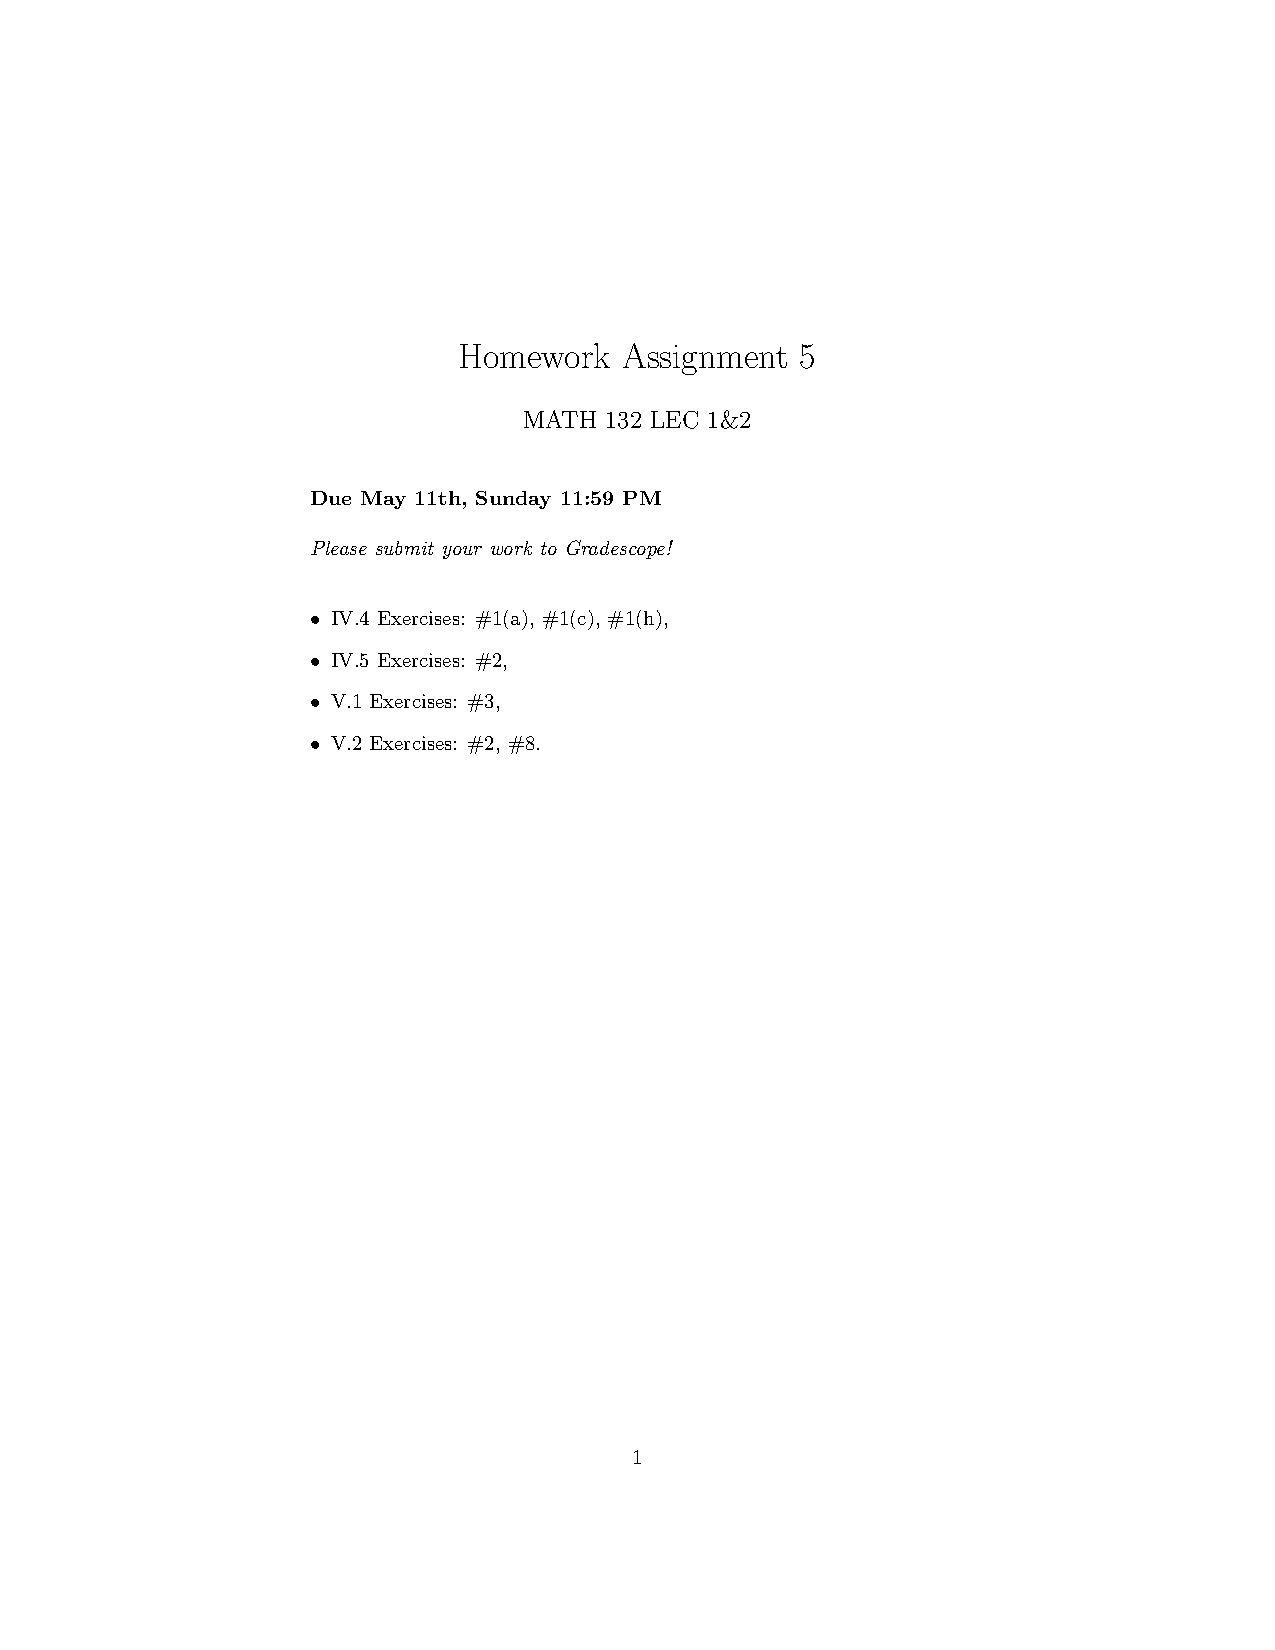
\includepdf[pages=-]{assignment.pdf}

\end{document}
